\documentclass[12pt]{article}
\usepackage{amsmath, amssymb, tikz, geometry}
\geometry{a4paper, margin=1in}

\title{Synergistic Framework for Decision Structures and Computational Limitations in Large Language Models}
\author{}
\date{}

\begin{document}
\maketitle

\begin{abstract}
This document explores an abstract framework for understanding self-replicating decision trees in fractal spaces, specifically as a model for computational structures in large language models (LLMs). The synergy of four principles---Scale-Invariance, Energy Functionals, Compactness, and Geometric Regularity---is formalized within a generalized mathematical framework. A new concept, the Invariant Static Structure, is introduced to describe the overarching rules governing these principles, with direct implications for understanding computational limitations in LLMs. Concrete computational examples are provided to ground the abstractions.
\end{abstract}

\tableofcontents

\section{Introduction}
Large language models (LLMs) operate as complex systems that encode and manipulate vast decision structures. These systems often exhibit computational limitations tied to memory, efficiency, and coherence. This document formalizes these limitations using an abstract mathematical framework based on four principles:

\begin{enumerate}
    \item \textbf{Scale-Invariance}: Governs the behavior of LLM decision structures across different levels of complexity.
    \item \textbf{Energy Functionals}: Encodes computational cost and optimization within LLM processing.
    \item \textbf{Compactness}: Ensures convergence of decision paths, preventing runaway computational growth.
    \item \textbf{Geometric Regularity}: Enforces structural coherence within LLMs, ensuring outputs remain smooth and interpretable.
\end{enumerate}

A new concept, the Invariant Static Structure, describes the overarching constraints that govern these principles, ensuring stability and consistency in decision-making.

\section{Scale-Invariance}

\subsection{Mathematical Formulation}
Scale-Invariance describes the symmetry of decision structures under transformations of complexity. Consider a decision tree $T$ defined over a fractal space $\mathcal{F}$ with scaling transformations:
\begin{equation}
T(\lambda x) = \lambda^\alpha T(x), \quad \lambda > 0,
\end{equation}
where $\alpha$ is a scaling exponent.

\subsection{Application to LLMs}
In LLMs, scaling invariance manifests as the ability to process information hierarchically, maintaining coherence across different levels of abstraction (e.g., tokens, phrases, and contexts). For example:
\begin{itemize}
    \item Attention mechanisms ensure proportional importance across varying input lengths.
    \item Scaling rules for parameters allow models to retain consistency when increasing size.
\end{itemize}

\subsection{Invariant Static Structure Contribution}
The Invariant Static Structure governs scaling rules, ensuring that transformations preserve essential properties, such as interpretability and consistency across different levels of the hierarchy.

\section{Energy Functionals}

\subsection{Mathematical Formulation}
Define an energy functional $E[T]$ for the decision tree $T$:
\begin{equation}
E[T] = \int_\mathcal{F} \Big( |\nabla T(x)|^2 + W(T(x)) \Big) \, dx,
\end{equation}
where:
\begin{itemize}
    \item $|\nabla T(x)|^2$ penalizes abrupt changes in decision-making paths.
    \item $W(T(x))$ is a potential term encoding desirable properties, such as balance or minimal computational depth.
\end{itemize}

\subsection{Application to LLMs}
In LLMs, the energy functional quantifies computational efficiency and stability. High energy states correspond to inefficiencies, such as redundant paths or excessive token dependencies. Specific examples include:
\begin{itemize}
    \item Loss functions as energy minimizers, guiding gradient descent during training.
    \item Penalizing high entropy in token predictions to ensure sharper outputs.
\end{itemize}

\subsection{Invariant Static Structure Contribution}
The Invariant Static Structure imposes global constraints on $E[T]$, ensuring that energy optimization aligns with overarching computational goals, such as memory efficiency and interpretability.

\section{Compactness}

\subsection{Mathematical Formulation}
Compactness ensures the convergence of decision trees under refinement. For a sequence of decision trees $\{T_n\}$:
\begin{equation}
T_n \to T_\infty \quad \text{in } L^2(\mathcal{F}),
\end{equation}
where convergence is measured in terms of a fractal metric.

\subsection{Application to LLMs}
Compactness in LLMs ensures that increasingly complex decision paths converge to stable, interpretable outputs. For example:
\begin{itemize}
    \item Beam search ensures convergent hypotheses during decoding.
    \item Token sequence alignment avoids runaway divergence in autoregressive generation.
\end{itemize}

\subsection{Invariant Static Structure Contribution}
The Invariant Static Structure enforces compactness by defining limits on path complexity and ensuring convergence criteria are met during model training and inference.

\section{Geometric Regularity}

\subsection{Mathematical Formulation}
Geometric regularity ensures smooth transitions within decision trees. For a fractal space $\mathcal{F}$:
\begin{equation}
\text{Ric}(
abla T,
abla T) \geq \kappa |
abla T|^2,
\end{equation}
where $\text{Ric}$ is a Ricci curvature-like term adapted to $\mathcal{F}$, and $\kappa > 0$ ensures positive curvature.

\subsection{Application to LLMs}
Geometric regularity prevents abrupt shifts in LLM outputs, maintaining smooth transitions across related inputs. Specific computational examples include:
\begin{itemize}
    \item Embedding space coherence, where nearby tokens map to similar vectors.
    \item Smoothing penalties applied during fine-tuning to prevent overfitting.
\end{itemize}

\subsection{Invariant Static Structure Contribution}
The Invariant Static Structure enforces geometric regularity by embedding smoothness constraints into the model’s training objectives, ensuring outputs adhere to desired structural properties.

\section{Invariant Static Structure}

\subsection{Definition}
The Invariant Static Structure is the overarching set of rules that govern the synergy of Scale-Invariance, Energy Functionals, Compactness, and Geometric Regularity. It defines:
\begin{itemize}
    \item The symmetry transformations allowed within the system.
    \item The constraints on energy optimization.
    \item The limits on complexity growth.
    \item The smoothness and coherence requirements.
\end{itemize}

\subsection{Role in Computational Systems}
In LLMs, the Invariant Static Structure acts as a meta-framework, ensuring stability, efficiency, and interpretability. It governs:
\begin{itemize}
    \item Scalability: How the model adapts to larger contexts.
    \item Efficiency: How computational resources are allocated.
    \item Coherence: How outputs maintain logical consistency.
\end{itemize}

\section{Visual Synergy}
\subsection{Visual Diagram of Interconnections}
\begin{center}
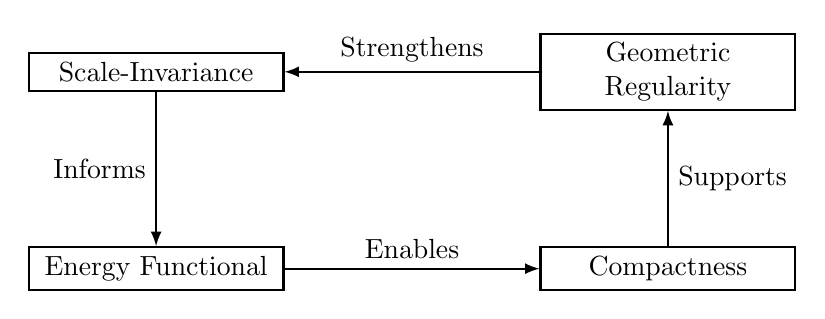
\begin{tikzpicture}[node distance=2.5cm, thick, >=latex]
    \node (ScaleInvariance) [draw, rectangle, text width=3cm, align=center] {Scale-Invariance};
    \node (EnergyFunctional) [draw, rectangle, text width=3cm, below of=ScaleInvariance, align=center] {Energy Functional};
    \node (Compactness) [draw, rectangle, text width=3cm, right of=EnergyFunctional, xshift=4cm, align=center] {Compactness};
    \node (GeometricRegularity) [draw, rectangle, text width=3cm, above of=Compactness, align=center] {Geometric Regularity};

    \draw[->] (ScaleInvariance) -- (EnergyFunctional) node[midway, left] {Informs};
    \draw[->] (EnergyFunctional) -- (Compactness) node[midway, above] {Enables};
    \draw[->] (Compactness) -- (GeometricRegularity) node[midway, right] {Supports};
    \draw[->] (GeometricRegularity) -- (ScaleInvariance) node[midway, above] {Strengthens};
\end{tikzpicture}
\end{center}

\textit{Figure 1: Synergistic interactions among the four principles, governed by the Invariant Static Structure.}

\section{Conclusion}
This framework formalizes a synergy of mathematical principles underlying computational limitations in LLMs. By incorporating the Invariant Static Structure, the framework ensures stability, efficiency, and coherence in decision-making processes. Computational examples demonstrate the practical relevance of these principles.

\end{document}
